\addchapheadtotoc

\chapter{Background}
In this chapter, we will begin to introduce the fundamentals of quantum mechanics with the Schr\"odinger equation. We will justify the extension of the Schr\"odinger equation to the Gross-Pitaevskii equation for Bose-Einstein condensates. Next, we will introduce the mathematical description of chaos and how chaos can be characterized with Lyapunov exponents. Numerical methods will be introduced, which will later be applied to the nonlinear Schr\"odinger equation to evolve it using computer simulation.

\section{Schr\"odinger equation}
The Schr\"odinger equation is mathematical description of how quantum mechanical objects evolve through time and space. It asserts that quantum objects are governed by a wave nature calculable with a differential equation in complex space. This wave is used to calculate the probability of the object existing in a particular location at a time. The equation takes form as a second order linear partial differential equation, defined in one-dimension as \begin{equation}
	i \hbar \pdv{t} \Psi(x, t) = \braket{x}{\hat{H} \Psi} = \left[ -\frac{\hbar^2}{2m} \pdv[2]{x} + V(x, t)\right] \Psi(x, t), \label{eq:tdse}
\end{equation}
for a wavefunction $\Psi(x, t)$ and a potential $V(x, t)$. This equation is the \textit{time-dependent} Schr\"odinger equation. For a constant potential in time and an assumption of separability, we can manipulate \eqref{eq:tdse} and define the \textit{time-independent} Schr\"odinger equation as \begin{equation}
	E \Psi(x) = \braket{\hat{H} x}{\Psi} = \left[ -\frac{\hbar^2}{2m} \pdv[2]{x} + V(x) \right] \Psi(x).
\end{equation}
We will now turn to approximations made using DFT with the Gross-Pitaevskii equation, simplifying the Schr\"odinger equation for the many-particle case of bosonic gases.
%If we take an example of an electron in the vicinity of another electron in one-dimension and account for Coulomb forces, the potential will be proportional to $1/x$. For a system of $N$-many electrons, the time-independent Schr\"odinger equation for one electron will take the form \[
%	E \psi_i(x) = \left[-\frac{\hbar^2}{2m_e} \pdv[2]{x} - \frac{e^2}{4\pi \epsilon_0} \sum_i^N \frac{1}{d_i}\right] \psi_i(x),
%\]
%for a distance between particles $d_i$. The potential term contains a sum over the distance of all particles. This becomes computationally problematic for the many-particle case, as it requires a wavefunction of $N$-variables, i.e. \[
%	\Psi(t, x_1, x_2, \dots, x_N) = \prod_{i=1}^{N} \psi_i.
%\]
%

\section{Gross-Pitaevskii equation}
As the Schr\"odinger equation describes one object, it becomes impractical to use it to model multiple interacting objects. This is due to the sheer number of variables in the wavefunction with the addition of each particle. The Gross-Pitaevskii equation (GPE) is approximation the many-particle Sch\"odinger equation for Bose-Einstein condensates (BECs) with the addition of a nonlinear term \cite{Barenghi_2016}. 
This model makes several assumptions to achieve lower complexity in the many-body Schr\"odinger equation.
First, this model assumes that the particles are about the same and do not interact strongly, and allows for the omission of quantum fluctuation effects. This many-body wavefunction is well-approximated by a collective product wavefunction.  These approximations allow a macroscopic many-body Sch\"odinger equation of form \begin{equation}
	i \hbar \pdv{\Psi}{t} = \left[ -\frac{\hbar^2}{2m} \pdv[2]{x} + V(x, t) + g \abs{\Psi}^2 \right] \Psi.  \label{eq:gpe}
\end{equation}
In the equation, note the addition of the nonlinear term with coupling constant $g$. This constant in one-dimension is given by \begin{equation}
	g = \frac{\hbar^2 a_s}{m},
\end{equation}
where $a_s$ is the s-wave scattering length characterizing atomic interactions in the low energy limit \cite{pethick2002bose}. This value can be determine experimentally, with $^{87}\text{Rb}$ and $^{23}\text{Na}$ having $a_s = \SI{5.8}{\nm}$ and $\SI{2.8}{\nm}$ respectively \cite{Barenghi_2016}. Additionally, as this is a macroscopic wavefunction, the normalization is now the number of particles in the condensate, i.e. \begin{equation}
	N = \int \abs{ \Psi }^2 \dd{x}.
\end{equation}
Solutions of the GPE are complex functions for an ensemble of classical particles, rather than functions of $N$-particles in the Schr\"odinger equation. It can be shown that solutions of the GPE are approximate solutions of the many-body Schr\"odinger equation for non-interacting bosons in the ground state. In the limit of $g=0$, the particles will have independent solutions to the Schr\"odinger equation.

\section{Chaos and Lyapunov exponents}
Chaos is a term commonly used in everyday speech, but can be hard to define mathematically. In the classic example of the double pendulum, a pendulum is connected to the tail of another pendulum. When we pull the pendulum up and drop the end, it creates a unique deterministic path based on the starting point. If we ever-so-slightly change the starting position, it creates a new unique path that may be wildly different than the last. This system can be completely deterministic, yet exhibit chaos and unpredictability. Chaos is found in unstable systems, where similar initial conditions can lead to wildly different outcomes. This can be characterized mathematically using Lyapunov exponents. 

Lyapunov exponents of a dynamical system tracks the rate of separation of two initially similar trajectories. The maximal Lyapunov exponent (MLE) along vector $\mathbf{Z}(t)$ perturbed from initial vector $\mathbf{Z}_0$ is defined as \begin{equation}
	\lambda = \lim_{t \to \infty} \lim_{\abs{\delta \mathbf{Z}_0} \to 0} \frac{1}{t} \ln\frac{\abs{\delta \mathbf{Z}(t)}}{\abs{\delta \mathbf{Z}_0}}.
\end{equation}

A well-known example of Lyapunov exponents is found in the Lorenz system. This system consists of a set of interdependent nonlinear differential equations, initially used to model atmospheric convection \cite{DeterministicNonperiodicFlow}. Typically for the Lorenz attractor, two lobes are seen, shown in Figure \ref{fig:lorenzattractor}. There exists points between the two lobes that is unstable, where minuscule changes along the curve will lead to the system switching or oscillating between the lobes. This is seen in Figure \ref{fig:lorenzexp}, where an initial point is perturbed slightly, and the distances between the two points is measured through time. An approximation of the maximal Lyapunov exponent is shown in the dashed red line. 

\begin{figure}[p]
	\centering
	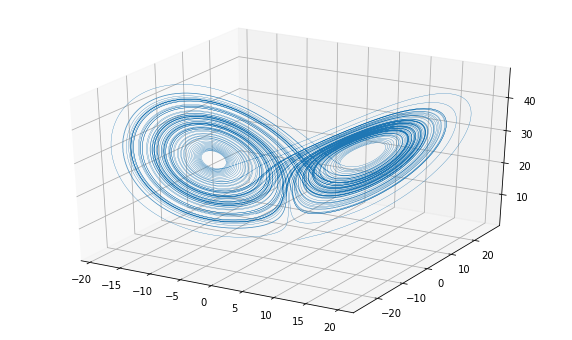
\includegraphics[width=0.7\linewidth]{chapter2/lorenzattractor}
	\caption[Three-dimensional plot of the Lorenz system.]{The Lorenz attractor in three dimensions with parameters $\sigma = 10$, $\beta = 8/3$, $\rho = 28$.}
	\label{fig:lorenzattractor}
\end{figure}

\begin{figure}[p]
	\centering
	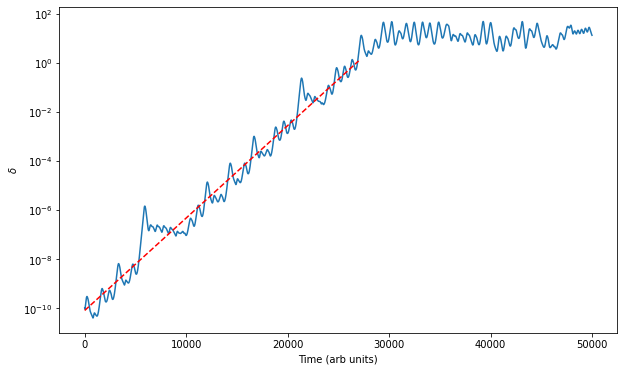
\includegraphics[width=0.7\linewidth]{chapter2/lorenzexp}
	\caption[Lyapunov exponent graphical approximation of the Lorenz system.]{The difference in trajectories through time of two nearby points, with an approximation of the MLE (dashed red). The plateau near the top is due to the maximal separation possible from the constraints of the system. }
	\label{fig:lorenzexp}
\end{figure}

\subsubsection{Lyapunov exponents in Hilbert space}
In order to find Lyapunov exponents in Hilbert space as required for quantum wavefunctions, we must devise a metric to find calculate distances. The norm of the wavefunctions is an obvious choice for this and has been used in prior works \cite{PhysRevA.83.043611}. This distance metric follows \begin{align}
	d^{(2)}(\psi_1, \psi_2; t) & = \frac{1}{2} \braket{\psi_1 - \psi_2}{\psi_1 - \psi_2} = \frac{1}{2} \int \dd{x} \abs{\psi_1(x, t) - \psi_2(x, t)}^2 \notag \\
		& = \int \dd{x} \left( \abs{\psi_1}^2 + \abs{\psi_2}^2 - 2 \psi_1^* \psi_2 \right). \label{eq:dist}
\end{align}
This metric will used in this paper to calculate distances between wavefunctions when determining the approximate maximal Lyapunov exponent. Note that as this is not a single trajectory and not in a phase space, this metric is an analogy to the maximal Lyapunov exponent. In the remainder of this work, we will refer to this metric as the Lyapunov exponent.


\section{Numerical methods}
%Numerical methods are procedures to solve a numerical problem, like finding solutions to a differential equation.
To see how the GPE evolves in time, the continuous spatial and time components must first be split into many smaller discrete slices---this is known as \textit{discretization}. Discretization has an innate error, growing for every increase in slice size. This error can be reduced by choosing minimized spatial and time deltas that adequately fit the problem, a trade-off with requiring excessive computational resources.

In this paper, we will use Runge-Kutta (RK) methods for approximating solutions of the GPE by solving the differential equation in time. To use this method, the spatial component must first be discretized using matrices described in Chapter 3. We will use the \texttt{solve\_ivp} function provided by SciPy as an implementation of the explicit Runge-Kutta method of order 5. This function has controllable tolerances, allowing an estimation of an error due to temporal discretization. 